\begin{savequote}[45mm]
\ascii{Any fool can write code that a computer can understand. Good programmers write code that humans can understand.}
\qauthor{\ascii{- Martin Flower}}
\end{savequote}

\chapter{算法骨架} 
\label{ch:skeleton}

\begin{content}

\end{content}

\section{前置}

\begin{content}

一般地,在执行测试前需要预置\ascii{setUp}实施测试环境的初始化工作,完成资源的准备。对既有的用例实施重构。

\subsection{测试用例}

\begin{leftbar}
 \begin{c++}[caption={\ttfamily{test/mars/core/TestCaseSpec.cc}}]
#include <gtest/gtest.h>
#include "mars/core/TestCase.h"

namespace {
  struct SimpleTest : TestCase {
    bool wasSetUp = false;
    bool wasRun = false;

  private:
    void setUp() override {
      wasSetUp = true;
    }

    void runTest() override {
      wasRun = true;
    }
  };
}

TEST(SimpleTest, make_sure_test_case_can_run_normally) {
  SimpleTest test;
  test.run();

  ASSERT_TRUE(test.wasSetUp);
  ASSERT_TRUE(test.wasRun);
}
 \end{c++}
\end{leftbar}

\subsection{通过编译}

重构\ascii{TestCase},仅公开\ascii{run}方法,并移除运行时多态的特性,它负责组织用例执行运行时的算法骨架。搬迁运行时多态行为至私有的两个虚函数,用户根据自己的场景定制\ascii{setUp}与\ascii{runTest},分别完成测试准备,及其测试执行。

\begin{leftbar}
 \begin{c++}[caption={\ttfamily{include/mars/core/TestCase.h}}]
struct TestCase {
  virtual ~TestCase() {}

  void run();

private:
  virtual void setUp() {}
  virtual void runTest() {}
};
  \end{c++}
\end{leftbar}

\subsection{通过测试}

实现\ascii{TestCase::run}的主体逻辑。

\begin{leftbar}
 \begin{c++}[caption={\ttfamily{src/mars/core/TestCase.cc}}]
#include "mars/core/TestCase.h"

void TestCase::run() {
  setUp();
  runTest();
}
 \end{c++}
\end{leftbar}

测试通过。

\end{content}

\section{后置}

\begin{content}

\subsection{测试用例}

同理,测试执行后使用\ascii{tearDown}完成现场清理,释放资源。用户通过定制私有的虚函数\ascii{tearDown}完成此功能。

\begin{leftbar}
 \begin{c++}[caption={\ttfamily{test/mars/core/TestCaseSpec.cc}}]
#include <gtest/gtest.h>
#include "mars/core/TestCase.h"

namespace {
  struct SimpleTest : TestCase {
    bool wasSetUp = false;
    bool wasRun = false;
    bool wasTearDown = false;

  private:
    void setUp() override {
      wasSetUp = true;
    }

    void runTest() override {
      wasRun = true;
    }

    void tearDown() override {
      wasTearDown = true;
    }
  };
}

TEST(SimpleTest, make_sure_test_case_can_run_normally) {
  SimpleTest test;
  test.run();

  ASSERT_TRUE(test.wasSetUp);
  ASSERT_TRUE(test.wasRun);
  ASSERT_TRUE(test.wasTearDown);  
}
 \end{c++}
\end{leftbar}

\subsection{通过编译}

当用例执行完成后,\ascii{TestCase::tearDown}负责清理现场。

\begin{leftbar}
 \begin{c++}[caption={\ttfamily{include/mars/core/TestCase.h}}]
struct TestCase {
  virtual ~TestCase() {}

  void run();

private:
  virtual void setUp() {}
  virtual void runTest() {}
  virtual void tearDown() {}
};
  \end{c++}
\end{leftbar}

\subsection{通过测试}

至此,完成了运行一个用例的主干逻辑,但缺乏异常处理机制,留待后续处理。

\begin{leftbar}
 \begin{c++}[caption={\ttfamily{src/mars/core/TestCase.cc}}]
#include "mars/core/TestCase.h"

void TestCase::run() {
  setUp();
  runTest();
  tearDown();
}
 \end{c++}
\end{leftbar}

\end{content}

\section{算法骨架}

\begin{content}

\ascii{TestCase::run}实现了\ascii{xUnit}最核心的高层算法逻辑,实现了高层算法逻辑与底层实现细节的解耦,并且实现了高层算法逻辑的高度复用。如\refig{simple-test}所示。

\begin{figure}[H]
\centering
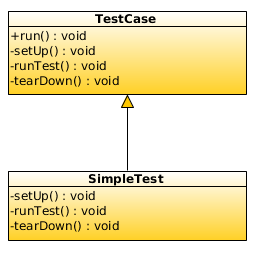
\includegraphics[width=0.4\textwidth]{figures/xunit/simple-test.png}
\caption{模板方法:定义算法骨架}
 \label{fig:simple-test}
\end{figure}

\subsection{引入策略}

模板方法模式与策略模式都可以用来分离高层的算法与具体的实现细节。之前已经看到了模板方法的实现,接下来探讨策略模式实现的效果,并从中对比两者之间的差异,从而指导设计的权衡与取舍。

\subsubsection{测试用例}

\ascii{TestCase}作为\ascii{TestCaseRunner}的抽象策略。新增测试用时,覆写\ascii{TestCase}相关接口,实现具体实现细节。

\begin{leftbar}
 \begin{c++}
namespace {
  struct SimpleTest : TestCase {
    bool wasSetUp = false;
    bool wasRun = false;
    bool wasTearDown = false;

  private:
    void setUp() override {
      wasSetUp = true;
    }

    void runTest() override {
      wasRun = true;
    }

    void tearDown() override {
      wasTearDown = true;
    }
  };
}

TEST(SimpleTest, run_test_case_using_strategry) {
  SimpleTest test;
  TestRunner runner(test);
  runner.run();

  ASSERT_TRUE(test.wasSetUp);
  ASSERT_TRUE(test.wasRun);
  ASSERT_TRUE(test.wasTearDown);  
}
 \end{c++}
\end{leftbar}

\subsubsection{通过测试}

\ascii{TestRunner::run}负责组织高层算法逻辑,算法子步骤的实现通过抽象的\ascii{TestCase}委托给某个具体策略对象完成。从而实现了\ascii{TestCaseRunner}与\ascii{SimpleTest}之间的解耦,两者都依赖于抽象的\ascii{TestCase},如\refig{simple-test-strategry}所示。

\begin{figure}[H]
\centering
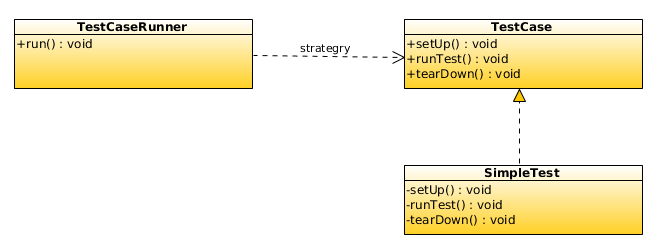
\includegraphics[width=1.0\textwidth]{figures/xunit/simple-test-strategry.png}
\caption{策略对象:定义算法骨架}
 \label{fig:simple-test-strategry}
\end{figure}


\begin{leftbar}
 \begin{c++}
struct TestCase {
  virtual ~TestCase() {}

  virtual void setUp() {}
  virtual void runTest() {}
  virtual void tearDown() {}
};

struct TestCaseRunner {
  TestCaseRunner(TestCase& test) : test(test) {
  }

  void run() {
    test.setUp();
    test.runTest();
    test.tearDown();
  }

private:
  TestCase& test;
};
 \end{c++}
\end{leftbar}

\subsection{权衡利弊}

使用模板方法,\ascii{SimpleTest}通过继承方式直接复用了\ascii{TestCase::run}高层算法逻辑。但继承是一种强依赖,增强了\ascii{SimpleTest}与\ascii{TestCase}之间的耦合关系。

使用策略方法,\ascii{TestCaseRunner}高层算法逻辑与\ascii{SimpleTest}是解耦的,但额外地引入类\ascii{TestCaseRunner}。

既然两个方案都有优缺点,到底应该采用哪个方案呢?其一,使用策略方法,需要建立额外的委托关系,不仅增加过多的类,使得设计变得更加复杂。其二,观察\ascii{TestCaseRunner::run}的实现,其实现基本完全委托给了\ascii{TestCase};按照迪米特法则,这段高层算法逻辑应该归属于\ascii{TeseCase}。

\begin{leftbar}
\begin{c++}
void TestCaseRunner::run() {
  test.setUp();
  test.runTest();
  test.tearDown();
}
\end{c++}
\end{leftbar}

按照这个推理,实施重构将\ascii{TestCaseRunner::run}搬迁至\ascii{TestCase},\ascii{TestCaseRunner}就成为一个空类,根本就没有存在的理由。因此,按照迪米特法则,也应优选模板方法。

如果优选模板方法,那么需要分析一下此场景使用模板方法的带来的副作用。无非就是因为引入继承关系从而增强了\ascii{TestCase}与\ascii{SimpleTest}的耦合关系。但是,考虑到\ascii{SimpleTest}是\ascii{xUnit Mars}最小调度单位,不会进一步被继承或组合而被复用,这个耦合关系仅局部于\ascii{SimpleTest}内部,不会被传播到其他地方,这是完全可以接受的设计。



\end{content}
